\documentclass[14pt,a4paper]{article}
\usepackage[slovak]{babel}
\usepackage{cite}
\usepackage[utf8]{inputenc}
\usepackage{graphicx}
\usepackage{url} % príkaz \url na formátovanie URL
\usepackage{hyperref}
\pagestyle{headings}

\title{Gamifikácia v informačných technológiach~\thanks{Semestrálny projekt v predmete Metódy inžinierskej práce, ak. rok 2022/23, vedenie: Ing. Richard Marko, PhD.}}

\author{Leonid Gurulev\\[2pt]
	{\small Slovenská technická univerzita v Bratislave}\\
	{\small Fakulta informatiky a informačných technológií}\\
	{\small \text{qgurulev@stuba.sk}}
	}

\date{\small 30. december 2022}


\begin{document}
\maketitle
\section{Úvod}
V tomto článku sa budeme zaoberať možnosťami gemifikácie v oblasti informatiky, 
kde sa pridaním herných prvkov do štúdia a vývoja informačných technológií 
a programovania uľahčilo štúdium programovania a informatiky pre mnohých ľudí, 
rovnako, ako sa gemifikáciou programov na písanie kódu 
a ich jednoduchším používaním uľahčilo písanie kódu pre 
akúkoľvek oblasť života alebo len pre potrebu 
či len tak na hranie. 
Keďže gemifikácia sa uplatňuje všade a vo všetkých sférach, 
bude sa skúmať, či je dobrá a či pribúda programátorov 
a mladých ľudí, ktorých život sa čoraz viac mení na hru, 
a či je dobrá pre tých, ktorí ju majú radi.




\section{Čo je gemifikácia?}
Gamifikácia je aplikácia prvkov herného dizajnu 
herných princípov v neherných kontextoch \cite{8166715}.
Možno ju definovať aj ako súbor činností a procesov na riešenie problémov 
pomocou alebo uplatnením vlastností herných prvkov \cite{gamify}.
Hry a prvky podobné hrám sa používajú na vzdelávanie, 
zábavu a zapájanie už tisíce rokov. Niektoré klasické herné prvky 
sú: body, odznaky a rebríčky.
Aby bolo jasné, gamifikácia nie je hra, 
ale aplikácia herného myslenia na vašu značku, podnik alebo organizáciu. 
Samotné hranie hier stimuluje ľudský mozog (uvoľňuje dopamín) a teraz možno osvedčené herné mechanizmy preniesť do marketingu a najmä do mobilného marketingu. Jeho argumentom je, že hry sú o potešení a že potešenie je nový marketing, jeden rozmer, ktorý je podľa neho mimoriadne silný.
Pre obchodníkov to nie je nič nové: vernostné programy (spôsob, 
ako získať preferencie spotrebiteľov pre podobné produkty) sa zameriavajú 
na hru prostredníctvom zhromažďovania bodov\cite{smarting}.
Gamifikácia sa v posledných rokoch uplatňuje v mnohých rôznych oblastiach. 
Jednou z týchto oblastí je vzdelávanie a odborná príprava, 
kde sa herné prvky využívajú na zvýšenie motivácie, 
angažovanosti a výkonnosti študentov. 
Gamifikácia je tiež ústrednou súčasťou návrhu mnohých 
mobilných aplikácií pre smartfóny a tablety v snahe 
dosiahnuť väčšie zapojenie používateľov a rozšírenie aplikácií. 
Predmetom gamifikácie sa stali aj podnikové webové 
stránky orientované na zákazníkov, 
ktoré sa snažia zlepšiť zákaznícku skúsenosť na webovej 
stránke. Gamifikácia sa uplatnila aj v podnikovom 
prostredí v snahe zlepšiť výsledky zamestnancov pri 
rozvoji ich každodenných úloh a práce\cite{gamifsoft}.


\section{Gamifikácia v softvérovom inžinierstve}
Gamifikácia sa snaží zlepšiť zapojenie používateľa, 
jeho motiváciu a výkon pri vykonávaní určitej úlohy; 
robí to prostredníctvom začlenenia herných mechaník a prvkov, 
čím sa táto úloha stáva atraktívnejšou. 
Aplikácia gamifikácie v softvérovom inžinierstve môže byť sľubná; 
softvérové projekty možno organizovať ako súbor úloh, 
ktoré možno zoradiť a ktoré treba splniť, 
na čo sú potrebné určité zručnosti a hlavne veľké kolektívne úsilie.
Oblasť softvérového inžinierstva zažíva v posledných rokoch pozitívny vývoj.
V posledných desaťročiach sa hlavná pozornosť sústredila na 
zlepšovanie softvérových procesov okrem iného pomocou noriem, 
ako sú CMMI alebo ISO 15504, začlenením agilného vývoja (najmä SCRUM) 
alebo podporou zlepšovania kvality produktov. 
Hlavným prínosom pri vývoji softvéru v porovnaní s inými 
disciplínami (výroba, priemyselné procesy) je však ľudský faktor, 
ktorého motivácia a zapojenie sú kľúčom k úspechu. 
Riadenie ľudí v softvérových projektoch sa považuje za kľúčovú otázku; 
to je prípad referenčných modelov, ako sú People CMM, 
Personal Software Process alebo Team Software Process. 
Napriek všetkým týmto snahám je však povaha úloh softvérového inžinierstva, 
ktoré sú zvyčajne nudné, faktorom, ktorý predstavuje hrozbu pre 
angažovanosť a motiváciu, a to tak na strane projektových manažérov, 
ako aj na strane členov tímu.
Na podporu tejto angažovanosti je dôležité vziať do úvahy, 
že softvérové projekty možno organizovať ako súbor úloh, 
ktoré možno zoradiť a ktoré treba splniť, 
na čo sú potrebné určité zručnosti a hlavne veľké kolektívne úsilie. 
Softvérové procesy môžu zahŕňať disciplínu a agilitu; 
softvérová kreativita sa tiež ukazuje ako racionálny prístup na 
kombináciu najlepších z týchto vlastností. 
Medzi softvérovým inžinierstvom a hrou možno preto zistiť 
dôležitú podobnosť: zahŕňajú činnosti, 
pri ktorých sa hráč učí nové zručnosti a používa a kombinuje ich 
na dosiahnutie určitých výziev, získava odmeny alebo dostáva tresty 
v závislosti od úspechu, resp. neúspechu .
Vzhľadom na tento kontext sa aplikácia gamifikácie v SE javí ako sľubná. 
Gamifikácia je všeobecne uznávaná ako "používanie prvkov herného dizajnu 
v neherných kontextoch". Gamifikácia využíva filozofiu, prvky a 
mechaniku herného dizajnu v neherných prostrediach na vyvolanie určitého 
správania ľudí, ako aj na zlepšenie ich motivácie a zapojenia do 
konkrétnej úlohy. To znamená, že gamifikácia preberá tie prvky, 
ktoré robia skutočné hry zábavnými a atraktívnymi (a dokonca návykovými), 
a využíva ich na zlepšenie skúseností hráčov v nehernom prostredí, 
napríklad na pracovisku, v škole, v softvérovej aplikácii alebo na 
webovej stránke orientovanej na zákazníka. 
Táto oblasť zaznamenala v posledných rokoch výrazný rast a popularitu.
V oblasti SE preto výskumníkom a odborníkom z praxe neunikli potenciálne 
výhody gamifikácie na pracovisku. 
Vývoj softvéru má zábavné aspekty, 
ale väčšina vývojárov softvéru považuje niektoré úlohy za nudné a zdĺhavé. 
Príkladom je kódovanie častí systému, ktoré sa opakujú
(napríklad kód pre prístup k údajom, 
ktorý je veľmi podobný pre všetky objekty domény), 
písanie jednotkových testov pre nie náročné funkcie alebo opravovanie ton 
jednoduchých problémov pri údržbe a iné. 
Gamifikácia umožňuje organizáciám explicitne odmeňovať vývojárov za 
každý aspekt ich práce, za každú splnenú úlohu, 
za každý napísaný unit test a za každý vyriešený problém. 
Mechanika gamifikácie nám poskytuje nielen spôsob, ako odmeňovať ľudí, 
ale môže dokonca urobiť prácu zábavnejšou. 
Sociálne prvky, ako sú spoločné úlohy alebo rebríčky, 
v ktorých vývojári alebo tímy porovnávajú svoj pokrok s pokrokom svojich 
partnerov, sú toho príkladom. Týmto spôsobom priebežne získavajú spätnú 
väzbu o hodnote svojej práce pre projekt a pre organizáciu. 
Zavedenie gamifikácie do každodennej práce softvérových inžinierov 
preto môže organizáciám zaoberajúcim sa vývojom softvéru pomôcť 
zlepšiť motiváciu a zapojenie vývojárov do ich práce, 
a tým aj výsledky softvérových projektov, a to z hľadiska kvality 
produktov aj výkonnosti projektu. 
Hoci sa táto práca zameriava najmä na spoločnosť a vývojárov, 
ktorí sa na procese zúčastňujú, prínosy začlenenia gamifikácie do 
SE sa týkajú spoločnosti ako organizácie, zamestnancov aj zákazníkov.
Začlenenie herných mechanizmov do nástrojov na podporu vývoja softvéru 
sa preto stalo súčasným trendom. 
Hlavnými prvkami gamifikácie, ktoré sú v takýchto nástrojoch nevyhnutné, 
sú: herné mechanizmy uplatňované v cykle výzvy - odmeny - tresty; 
odznaky alebo medaily, ktoré sa získavajú ako výsledok dosiahnutých 
úspechov, a spätná väzba o výkonnosti jednotlivcov a tímov 
v porovnaní s ostatnými. 
Aj existujúce komerčné nástroje začínajú podporovať procesy SE tým, 
že obsahujú uvedené základné mechanizmy gamifikácie; 
patria k nim napríklad Gamify, RedCritter, PropsToYou, 
ScrumKnowsy, Masterbranch, CodeHunt a pod\cite{201721}.

Na povzbudenie vývojárov k zdieľaniu vedomostí sa používajú aj 
techniky gamifikácie. 
V poslednom desaťročí sme boli svedkami vzostupu sociálnych médií, 
ako je Twitter, a sociálnych kódovacích platforiem, 
ako sú GitHub a StackOverflow\cite{8717887}.


\section{Preklady pouzitia}
%M. Lykke M. Coto S. Mora N. Vandel and C. Jantzen "Motivating programming students by problem based learning and LEGO robots" IEEE Global Engineering Education Conference (EDUCON) pp. 3-5 April 2014. 
Hra Agile Estimating and Planning Poker Game
\space
Tímy vyvíjajúce softvér môžu používať rôzne techniky na stanovenie priorít 
požiadaviek projektu - usporiadanie úloh podľa úrovne dôležitosti 
je jednou z najdôležitejších povinností tímu. 
Aj keď sa projekty začínajú s hviezdnym úspechom, nastane chvíľa, 
keď je potrebné rozhodnúť, ktoré požiadavky treba dokončiť a ktoré odložiť, 
aby bol produkt dodaný podľa časového plánu.
Vo fáze analýzy požiadaviek každý tím rozhoduje o relevantnosti a dôležitosti 
každej požiadavky tým, že odpovedá na realizovateľné otázky. 
Musia sa zohľadniť časovo-priestorové obmedzenia, 
dobre sa musia pochopiť a vypočítať zdroje, výdavky a možnosti chýb. 
Vždy sa musí počítať s ďalším dôležitým závažným problémom - klienti 
často menia svoje požiadavky aj v pokročilej fáze vývoja projektu. 
Zvyčajne majú klienti na začiatku len predstavu a detaily sa kujú až neskôr. 
Tomu sa treba vyhnúť, pretože to vedie k neuveriteľným komplikáciám v ďalšom 
priebehu vývoja. Tento jav je známy aj ako "metastáza možností" - keď sa 
funkcie aplikácie neustále rozrastajú do epických rozmerov.
Every task must be estimated before prioritization. 
The grading of the tasks is achieved by playing Poker Planning. 
Each of the teams starts the game and loads their user stories to be assessed. 
The grading is done through poker cards, where every card has a numeric value – weight.
The team manager gives the team start game, and every member of the team has 
to personally estimate every user story, after which the game analyses all 
user grades and calculates the average result. 
shows the online game (planitpoker.com), 
which is used by the students during class.
Pokerové plánovanie, známe aj ako Scrum Poker, je technika hodnotenia 
úsilia na základe konsenzu. 
Členovia tímu hodnotia používateľské príbehy hraním s 
virtuálnymi očíslovanými kartami, ktoré ostatní členovia tímu nevidia. 
Výsledky hlasovania pre každý používateľský príbeh sa odhalia po tom, 
ako všetci dokončia výber. Použitie takejto hry pomáha obísť 
psychologický efekt ukotvenia zaujatosti, ktorý sa vyskytuje pri 
hlasovaní hlasom - keďže existuje riziko vzájomného ovplyvňovania 
názorov vopred. Tento efekt môže viesť k nesprávnemu hodnoteniu a 
stanoveniu priorít úloh\cite{8757200}.
\begin{figure}[!h]
\centering
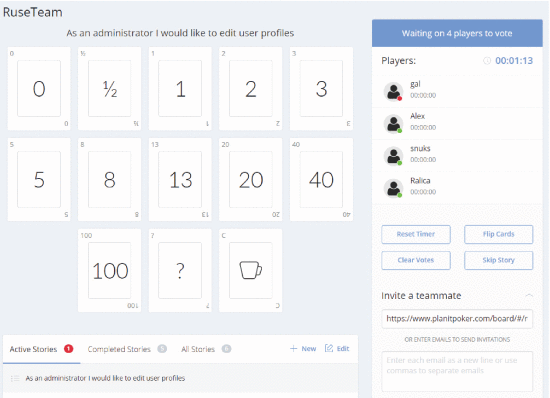
\includegraphics[width=0.5\textwidth]{planitpoker.png}
\caption{Planitpoker.com}
\label{fig:planitpoker}
\end{figure}

\section{Výhody a nevýhody gamifikácie}

\section{Štatistika}


\quad
\newpage

\bibliography{literatura}
\bibliographystyle{plain}
\end{document}
